\documentclass[conference,compsoc]{IEEEtran}
\usepackage[utf8]{inputenc}
%\usepackage{hyperref}
\usepackage{lipsum}
\usepackage{graphicx}
\usepackage[pdftex,
pdfauthor={Rene Kremer},
pdftitle={An Overview and Comparison of Designs of Architectures for Seamless System Reconfiguration},
pdfsubject={Overview and Comparison of Architectures like PERFoRM and PRIME in the field of the industrial revolution},
pdfkeywords={System Architecture, Seamless System Reconfiguration, Multi Agent System},
pdfproducer={PDFLatex},
pdfcreator={PDFLatex}]{hyperref}

% *** CITATION PACKAGES ***
%
\ifCLASSOPTIONcompsoc
  % IEEE Computer Society needs nocompress option
  % requires cite.sty v4.0 or later (November 2003)
  \usepackage[nocompress]{cite}
\else
  % normal IEEE
  \usepackage{cite}
\fi

% *** GRAPHICS RELATED PACKAGES ***
%
\ifCLASSINFOpdf
  % \usepackage[pdftex]{graphicx}
  % declare the path(s) where your graphic files are
  % \graphicspath{{../pdf/}{../jpeg/}}
  % and their extensions so you won't have to specify these with
  % every instance of \includegraphics
  % \DeclareGraphicsExtensions{.pdf,.jpeg,.png}
\else
  % or other class option (dvipsone, dvipdf, if not using dvips). graphicx
  % will default to the driver specified in the system graphics.cfg if no
  % driver is specified.
  % \usepackage[dvips]{graphicx}
  % declare the path(s) where your graphic files are
  % \graphicspath{{../eps/}}
  % and their extensions so you won't have to specify these with
  % every instance of \includegraphics
  % \DeclareGraphicsExtensions{.eps}
\fi
% graphicx was written by David Carlisle and Sebastian Rahtz. It is
% required if you want graphics, photos, etc. graphicx.sty is already
% installed on most LaTeX systems. The latest version and documentation
% can be obtained at: 
% http://www.ctan.org/pkg/graphicx
% Another good source of documentation is "Using Imported Graphics in
% LaTeX2e" by Keith Reckdahl which can be found at:
% http://www.ctan.org/pkg/epslatex
%
% latex, and pdflatex in dvi mode, support graphics in encapsulated
% postscript (.eps) format. pdflatex in pdf mode supports graphics
% in .pdf, .jpeg, .png and .mps (metapost) formats. Users should ensure
% that all non-photo figures use a vector format (.eps, .pdf, .mps) and
% not a bitmapped formats (.jpeg, .png). The IEEE frowns on bitmapped formats
% which can result in "jaggedy"/blurry rendering of lines and letters as
% well as large increases in file sizes.
%
% You can find documentation about the pdfTeX application at:
% http://www.tug.org/applications/pdftex





% *** MATH PACKAGES ***
%
%\usepackage{amsmath}
% A popular package from the American Mathematical Society that provides
% many useful and powerful commands for dealing with mathematics.
%
% Note that the amsmath package sets \interdisplaylinepenalty to 10000
% thus preventing page breaks from occurring within multiline equations. Use:
%\interdisplaylinepenalty=2500
% after loading amsmath to restore such page breaks as IEEEtran.cls normally
% does. amsmath.sty is already installed on most LaTeX systems. The latest
% version and documentation can be obtained at:
% http://www.ctan.org/pkg/amsmath





% *** SPECIALIZED LIST PACKAGES ***
%
%\usepackage{algorithmic}
% algorithmic.sty was written by Peter Williams and Rogerio Brito.
% This package provides an algorithmic environment fo describing algorithms.
% You can use the algorithmic environment in-text or within a figure
% environment to provide for a floating algorithm. Do NOT use the algorithm
% floating environment provided by algorithm.sty (by the same authors) or
% algorithm2e.sty (by Christophe Fiorio) as the IEEE does not use dedicated
% algorithm float types and packages that provide these will not provide
% correct IEEE style captions. The latest version and documentation of
% algorithmic.sty can be obtained at:
% http://www.ctan.org/pkg/algorithms
% Also of interest may be the (relatively newer and more customizable)
% algorithmicx.sty package by Szasz Janos:
% http://www.ctan.org/pkg/algorithmicx




% *** ALIGNMENT PACKAGES ***
%
%\usepackage{array}
% Frank Mittelbach's and David Carlisle's array.sty patches and improves
% the standard LaTeX2e array and tabular environments to provide better
% appearance and additional user controls. As the default LaTeX2e table
% generation code is lacking to the point of almost being broken with
% respect to the quality of the end results, all users are strongly
% advised to use an enhanced (at the very least that provided by array.sty)
% set of table tools. array.sty is already installed on most systems. The
% latest version and documentation can be obtained at:
% http://www.ctan.org/pkg/array


% IEEEtran contains the IEEEeqnarray family of commands that can be used to
% generate multiline equations as well as matrices, tables, etc., of high
% quality.




% *** SUBFIGURE PACKAGES ***
%\ifCLASSOPTIONcompsoc
%  \usepackage[caption=false,font=footnotesize,labelfont=sf,textfont=sf]{subfig}
%\else
%  \usepackage[caption=false,font=footnotesize]{subfig}
%\fi
% subfig.sty, written by Steven Douglas Cochran, is the modern replacement
% for subfigure.sty, the latter of which is no longer maintained and is
% incompatible with some LaTeX packages including fixltx2e. However,
% subfig.sty requires and automatically loads Axel Sommerfeldt's caption.sty
% which will override IEEEtran.cls' handling of captions and this will result
% in non-IEEE style figure/table captions. To prevent this problem, be sure
% and invoke subfig.sty's "caption=false" package option (available since
% subfig.sty version 1.3, 2005/06/28) as this is will preserve IEEEtran.cls
% handling of captions.
% Note that the Computer Society format requires a sans serif font rather
% than the serif font used in traditional IEEE formatting and thus the need
% to invoke different subfig.sty package options depending on whether
% compsoc mode has been enabled.
%
% The latest version and documentation of subfig.sty can be obtained at:
% http://www.ctan.org/pkg/subfig




% *** FLOAT PACKAGES ***
%
%\usepackage{fixltx2e}
% fixltx2e, the successor to the earlier fix2col.sty, was written by
% Frank Mittelbach and David Carlisle. This package corrects a few problems
% in the LaTeX2e kernel, the most notable of which is that in current
% LaTeX2e releases, the ordering of single and double column floats is not
% guaranteed to be preserved. Thus, an unpatched LaTeX2e can allow a
% single column figure to be placed prior to an earlier double column
% figure.
% Be aware that LaTeX2e kernels dated 2015 and later have fixltx2e.sty's
% corrections already built into the system in which case a warning will
% be issued if an attempt is made to load fixltx2e.sty as it is no longer
% needed.
% The latest version and documentation can be found at:
% http://www.ctan.org/pkg/fixltx2e


%\usepackage{stfloats}
% stfloats.sty was written by Sigitas Tolusis. This package gives LaTeX2e
% the ability to do double column floats at the bottom of the page as well
% as the top. (e.g., "\begin{figure*}[!b]" is not normally possible in
% LaTeX2e). It also provides a command:
%\fnbelowfloat
% to enable the placement of footnotes below bottom floats (the standard
% LaTeX2e kernel puts them above bottom floats). This is an invasive package
% which rewrites many portions of the LaTeX2e float routines. It may not work
% with other packages that modify the LaTeX2e float routines. The latest
% version and documentation can be obtained at:
% http://www.ctan.org/pkg/stfloats
% Do not use the stfloats baselinefloat ability as the IEEE does not allow
% \baselineskip to stretch. Authors submitting work to the IEEE should note
% that the IEEE rarely uses double column equations and that authors should try
% to avoid such use. Do not be tempted to use the cuted.sty or midfloat.sty
% packages (also by Sigitas Tolusis) as the IEEE does not format its papers in
% such ways.
% Do not attempt to use stfloats with fixltx2e as they are incompatible.
% Instead, use Morten Hogholm'a dblfloatfix which combines the features
% of both fixltx2e and stfloats:
%
% \usepackage{dblfloatfix}
% The latest version can be found at:
% http://www.ctan.org/pkg/dblfloatfix




% *** PDF, URL AND HYPERLINK PACKAGES ***
%
%\usepackage{url}
% url.sty was written by Donald Arseneau. It provides better support for
% handling and breaking URLs. url.sty is already installed on most LaTeX
% systems. The latest version and documentation can be obtained at:
% http://www.ctan.org/pkg/url
% Basically, \url{my_url_here}.




% *** Do not adjust lengths that control margins, column widths, etc. ***
% *** Do not use packages that alter fonts (such as pslatex).         ***
% There should be no need to do such things with IEEEtran.cls V1.6 and later.
% (Unless specifically asked to do so by the journal or conference you plan
% to submit to, of course. )


% correct bad hyphenation here
\hyphenation{op-tical net-works semi-conduc-tor}


\begin{document}
%
% paper title
% Titles are generally capitalized except for words such as a, an, and, as,
% at, but, by, for, in, nor, of, on, or, the, to and up, which are usually
% not capitalized unless they are the first or last word of the title.
% Linebreaks \\ can be used within to get better formatting as desired.
% Do not put math or special symbols in the title.
\title{An Overview and Comparison of Designs of Architectures for Seamless System Reconfiguration}


% author names and affiliations
% use a multiple column layout for up to three different
% affiliations
\author{\IEEEauthorblockN{René Kremer}
\IEEEauthorblockA{University of Lübeck\\
%Institute of Computer Engineering\\
Lübeck, Germany\\
Email: rene.kremer@student.uni-luebeck.de}}

% make the title area
\maketitle

\begin{abstract}
Driven by the fourth industrial revolution emerges a need for concepts, methods and technologies which will take on the new challenge of digitalization. In future systems digitalization is an important principle with the goal of processing and collecting large amounts of data as well as having smart, pluggable, cooperating and collaborating components. A special design process has to be addressed to allow building evolvable and complex systems for various requirements and use cases. This paper focuses on architectures like PERFoRM and the PRIME Framework for Multi Agent Systems (MAS) by comparing them, as both are trying to support the new upcoming system designs.
\end{abstract}

\section{Introduction} % first page
% no \IEEEPARstart

\lipsum[1-6]


\hfill rk

\hfill Juni 15, 2017

% no keywords

\IEEEpeerreviewmaketitle

\section{State of the Art Methodologies} % second page
In this section different approaches will be introduced, which are the results of successful projects. 

\subsection{Multi-Agent Systems}
Multi-Agent Systems (MAS) are an approach to develop an agent based decentralized control architecture for production systems. This allows an easy support for cyber-physical concepts and the creation of smart components as agents in the system. This means the production system is a collection of agents, where agents interact with each other. Every agent got an own action scope and is aware of the status of its surrounding agents. Therefore it is possible for them to self-organize in case of changes and disturbances, which means they reconfigure and operate accordingly to its environment \cite{HarmonizedSystems}.

\subsection{Plug and Produce Technology}
"Plug and Produce" technologies try to build modules, which can integrate intelligent components. This is accomplished by using standard interfaces and adapters for existing interfaces. Following this approach it is possible to use plug-and-produce devices, which could have built-in intelligence and profit of sensors and actors. These plug-and-produce devices might be used to integrate new capabilities to an existing production systems or a new one \cite{HarmonizedSystems}. Self*-Features possess an important role in these upcoming architectures \cite{SpecPERFoRM} and the "Plug and Produce" technology should focus on self-adaptive and reconfigurable components to support a flexible solution. MAS was used in some projects to accomplish plug-and-produce with self-adaption. PRIME, which was developed in scope of the PRIME project and funded by the European FP7 program, used a MAS in this context to support semi-automatical configuration through a human-machine-interface (HMI). Reconfiguration in the PRIME architecture is handled through different agent roles and enables the integration of legacy systems \cite{HarmonizedSystems}.

\subsection{Service-oriented Architecture}
Other projects researched the possible use of Service-oriented Architectures (SoA), which are mostly commonly used in the context of Web services. The principle of SoA could be used at a device and application level to enable and integrate distributed smart embedded systems. These components are handled as services, which are flexible parts in this kind of architecture. Therefore it is important to create an open and flexible environment that is extended by the scope of the collaborative SoA \cite{HarmonizedSystems}. This means that the industrial middleware needs to be able to discover and register new services and also expose functionalities of the heterogeneous components as services \cite{SpecPERFoRM}. Data transformation for these different services also needs to be handled by the middleware, which adds additional intelligence to this component. Once the groundwork is done, integration of new services and communication between existing ones can be simplified on different levels of the enterprise architecture. As services are interoperable and reusable this approach allows to develop self-learning production systems by using data mining and context awareness \cite{HarmonizedSystems}.


\subsection{Cloud Technology}
Towards the goal of developing an architecture that can be used in the context of industry 4.0 and its digitalization, the possible use of cloud technologies was investigated. Cloud technologies are used to build a common data model to integrate data of heterogeneous components together onto one platform. This allows the creation of a systematic knowledge generation ranging from design till usage phase by knowledge gathering and refining. Some projects even showed that SoA and Cloud technologies work hand in hand \cite{HarmonizedSystems}.  

\subsection{Conclusion}
Different solutions were developed for the new agile-manufacturing generation using agent-systems, (smart) component networks, service-oriented paradigms and cloud principles to overcome the challenges of the migration from traditional production systems towards cyber-physical-production-systems (CPPS) \cite{HarmonizedSystems}.

1. Integration: The problem posed by each of these solutions is the individual integration of existing components and legacy systems. Therefore a common interface and standard needs to be established for a wide use in different industries.

2. Support Businesses: It is not enough to develop new concepts and technologies if it is not benefiting the goal of businesses. Requirements and performance indicators needs to be analyzed to support those real business requirements and therefore improve the overall performance of the business.

3. Human Factor:  The human factor is a flexibility driver and therefore needs special attention. Not only highly usable HMIs need to be developed. The impact of these upcoming concepts and architectures needs to be analyzed and evaluated. Necessary skills for operators and maintainers possibly will change. Activities on education and training become important parts so that human workers can keep up with new state of the art procedures and technologies.

4. Maturity and Migration: These new approaches, which are currently state of the art, are not fully tested in industry. As the migration of new technologies will have a big impact on the production and expenses of a company a good and tested migration strategy needs to be developed. Special attention lies on the smooth integration of legacy systems.

\section{PRIME} % third page
\lipsum[1-10]
\section{PERFoRM} % fourth page
This section gives a brief introduction to PERFoRM, its requirements, assumptions and architectural elements.
\subsection{Requirements}
The PERFoRM project is funded by the European Unions Horizon 2020 research and innovation programme and investigates the requirements for new innovative production systems. PERFoRM does not try to develop a new architecture from scratch but instead tries to re-use the results of previous successful projects in this field \cite{SpecPERFoRM}. 
\subsection{Assumptions}
1. Integrate legacy systems: As most of the industry uses legacy systems the integration of these systems is an important part to consider. Standard interfaces for syntax and semantic define how to communicate with components of the system. Technology adapters connect existing components to these interfaces. Once these interfaces and adapters are commonly established heterogeneous components can be connected to the communication infrastructure, which can address other backbone level systems via Machine-to-Machine (M2M) and Enterprise-Service-Bus (ESB) technologies.

2. Integrate advanced planning and simulation applications: New CPPS are based on smart components. To support smart and self*-features of those devices it is essential to allow simulation and planning. This allows them to be agile and adaptive to its surroundings. A way to enable this is using MAS and cloud technologies to propagate strategies and decision making.

3. Seamless data representation: Keeping in mind that devices are mostly heterogeneous different representations of data need to be processed. An standard representation of industrial data models and gateways for data transformation on machinery and backbone level are needed to accomplish this problem.

4. Components and Configuration on the fly: Disturbances of the work-flow need to be recognized and handled. Distributed approaches, e.g. MAS or SoA, combined with registry and discovery mechanisms enable the architecture to support a plug-and-play approach for components. In case of disturbances, planned or not, e.g. maintenance or device failure, reconfiguration of running components might be necessary. Other projects, like PRIME, showed concepts to support reconfiguration and also self*-features in an productive environment.

5. Distributed and heterogeneous components: In addition to the before mentioned standard interfaces and technology adapters, service-oriented design principles like SoA allow a more abstract view of distributed and heterogeneous components. The system can expose functionalities as services and aggregate and composite those services. Therefore the combination of services can create new services and also describe services used for self-organization of smart components in the production system.

6. Intelligent production components: Components getting more powerful in terms of performance allow for decentralized intelligence. Artificial Intelligence methods, e.g. MAS, could be supported by these components. Data analysis could be handled on an advanced level to help the AI and their self*-features. An example would be the self-adaption in case a surrounding component fails. As these smart devices watch their surroundings and the status of other devices they can react to changes based on status or disturbances in another part of the work-flow.

7. Integrate Humans: Still with all those smart devices and innovative ways to enhance new performance peaks to satisfy customer needs, humans are a important part. With changing techniques and concepts human operators and maintainers need to adapt to those changes. HMI and mobile applications need to be highly usable and supportive. Education and Training activities need to take new ways to keep up with these upcoming technologies and enable humans to understand, operate and maintain them \cite{SpecPERFoRM}.
\subsection{Architectural Elements}
Based on the assumptions made by PERFoRM there are elements in the architecture which seem necessary.

The integration of legacy systems and communication between distributed heterogeneous components make standard interfaces and technology adapters essential.
Therefore standards for these interfaces and adapters need to be establish so that independent to specific manufacturers of devices and software components it is ensured that they fit into the architecture.

\begin{figure}[ht]
	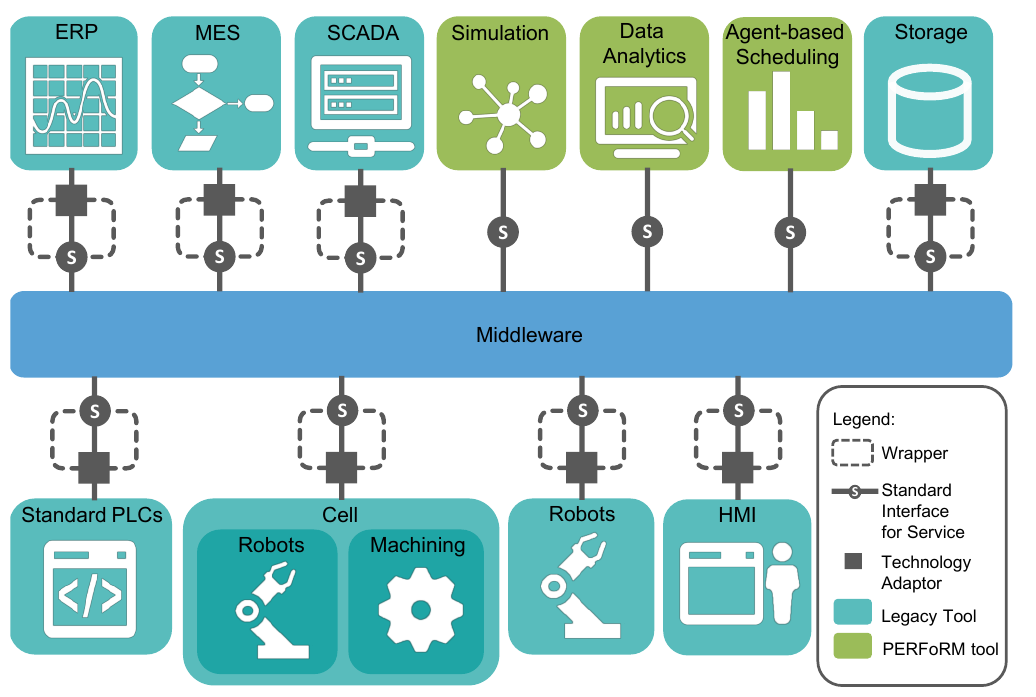
\includegraphics[width=\columnwidth]{img/PERFoRM-Architecture.png}
	\caption{The PERFoRM system architecture\cite{SpecPERFoRM}}
\end{figure}

Another important part of the architecture is an industrial middleware. To ensure seamless data representation, data transformation and approaches like MAS a smart middleware is needed. In terms of service-orientation these features are enriched with service registry and discovery. Depending on the chosen architecture design the middleware might be the central communication and organization hub for all other parts of the system.


\section{Comparison} % fifth to sixth page
\section{Conclusion} % sixth page
The conclusion goes here.

% use section* for acknowledgment
\ifCLASSOPTIONcompsoc
  % The Computer Society usually uses the plural form
  \section*{Acknowledgments}
\else
  % regular IEEE prefers the singular form
  \section*{Acknowledgment}
\fi

The authors would like to thank...

\begin{thebibliography}{1}

\bibitem{Hybrid}
Tiago Santos and Luis Ribeiro and Andre Dionisio Rocha and Jose Barata, \emph{A system reconfiguration architecture for hybrid
automation systems based in agents and
programmable logic controllers}, IEEE, 2016

\bibitem{SpecPERFoRM}
Paulo Leitão and José Barbosa and Arnaldo Pereira and José Barata  and Armando W. Colombo, \emph{Specification of the PERFoRM Architecture for the Seamless Production System Reconfiguration}, IEEE, 2016

\bibitem{HarmonizedSystems}
A. Calà and M. Foehr and D. Rohrmus and N. Weinert and O. Meyer and M. Taisch and F. Boschi and P. M. Fantini and P. Perlo and P. Petrali and J. Vallhagen, \emph{Towards Industrial Exploitation of Innovative and Harmonized Production Systems}, IEEE, 2016
\end{thebibliography}

% that's all folks
\end{document}

% An example of a floating figure using the graphicx package.
% Note that \label must occur AFTER (or within) \caption.
% For figures, \caption should occur after the \includegraphics.
% Note that IEEEtran v1.7 and later has special internal code that
% is designed to preserve the operation of \label within \caption
% even when the captionsoff option is in effect. However, because
% of issues like this, it may be the safest practice to put all your
% \label just after \caption rather than within \caption{}.
%
% Reminder: the "draftcls" or "draftclsnofoot", not "draft", class
% option should be used if it is desired that the figures are to be
% displayed while in draft mode.
%
%\begin{figure}[!t]
%\centering
%\includegraphics[width=2.5in]{myfigure}
% where an .eps filename suffix will be assumed under latex, 
% and a .pdf suffix will be assumed for pdflatex; or what has been declared
% via \DeclareGraphicsExtensions.
%\caption{Simulation results for the network.}
%\label{fig_sim}
%\end{figure}

% Note that the IEEE typically puts floats only at the top, even when this
% results in a large percentage of a column being occupied by floats.


% An example of a double column floating figure using two subfigures.
% (The subfig.sty package must be loaded for this to work.)
% The subfigure \label commands are set within each subfloat command,
% and the \label for the overall figure must come after \caption.
% \hfil is used as a separator to get equal spacing.
% Watch out that the combined width of all the subfigures on a 
% line do not exceed the text width or a line break will occur.
%
%\begin{figure*}[!t]
%\centering
%\subfloat[Case I]{\includegraphics[width=2.5in]{box}%
%\label{fig_first_case}}
%\hfil
%\subfloat[Case II]{\includegraphics[width=2.5in]{box}%
%\label{fig_second_case}}
%\caption{Simulation results for the network.}
%\label{fig_sim}
%\end{figure*}
%
% Note that often IEEE papers with subfigures do not employ subfigure
% captions (using the optional argument to \subfloat[]), but instead will
% reference/describe all of them (a), (b), etc., within the main caption.
% Be aware that for subfig.sty to generate the (a), (b), etc., subfigure
% labels, the optional argument to \subfloat must be present. If a
% subcaption is not desired, just leave its contents blank,
% e.g., \subfloat[].


% An example of a floating table. Note that, for IEEE style tables, the
% \caption command should come BEFORE the table and, given that table
% captions serve much like titles, are usually capitalized except for words
% such as a, an, and, as, at, but, by, for, in, nor, of, on, or, the, to
% and up, which are usually not capitalized unless they are the first or
% last word of the caption. Table text will default to \footnotesize as
% the IEEE normally uses this smaller font for tables.
% The \label must come after \caption as always.
%
%\begin{table}[!t]
%% increase table row spacing, adjust to taste
%\renewcommand{\arraystretch}{1.3}
% if using array.sty, it might be a good idea to tweak the value of
% \extrarowheight as needed to properly center the text within the cells
%\caption{An Example of a Table}
%\label{table_example}
%\centering
%% Some packages, such as MDW tools, offer better commands for making tables
%% than the plain LaTeX2e tabular which is used here.
%\begin{tabular}{|c||c|}
%\hline
%One & Two\\
%\hline
%Three & Four\\
%\hline
%\end{tabular}
%\end{table}


